\chapter{Interpretazione Astratta}

L'interpretazione astratta e' una tecnica di analisi statica. Estrae \emph{sistematicamente} proprietà dei programmi in modo \emph{approssimato} ma \emph{corretto}. Compare per la prima volta nel 1977 nel paper \cite{cousot} di P.~Cousot e R.~Cousot.

\section{Semantica dei linguaggi imperativi}

La nostra analisi avviene su programmi Javascript. Questo è un linguaggio ad oggetti, ed anche imperativo. I suoi sorgenti sono composti da istruzioni di controllo e assegnazione. Durante l'esecuzione del programma viene mantenuta una \emph{memoria} o \emph{store} che è un'associazione di tipo \emph{variabile\textrightarrow{}valore}. 

\begin{definition}[Semantica]
Si definisce semantica di un linguaggio l'insieme di regole che descrive il comportamento dei programmi scritti in tale linguaggio. Formalmente (secondo il formalismo denotazionale) è un insieme di funzioni del tipo
\[ \semantics{\texttt{costrutto}}(\sigma) = \sigma' \]
con $\sigma : \set{Variabili} \to \set{Valori}$.
\end{definition}

La semantica di Javascript, detta \emph{concreta} (in contrapposizione a quella approssimata che chiameremo \emph{astratta}) modella l'esecuzione delle espressioni, delle istruzioni di controllo e l'aggiornamento dello store $\sigma$. La semantica di Javascript e' descritta in \cite{javascriptsemantics}. 

\subsection{Point}

Si chiama \emph{point} (indicato con $ p \in \set{Point} $) l'oggetto che punta alla prossima istruzione da eseguire. In un certo istante nell'esecuzione del programma, ad un punto $p \in \set Point$, vale un certo store $\sigma \in \set Store$. 

\section{Collecting semantics}

\begin{definition}[Collecting semantics]
La \emph{collecting semantics} è una funzione del tipo
\[ \mathcal{C} : \set{Point} \to \set \wp(\set{Store}) \]
che associa ad un certo punto del programma tutti i possibili combinazioni di valori che la memoria può assumere.
\end{definition}

Tramite la nostra collecting semantics possiamo dimostrare la nostra proprietà vale o meno guardando lo store. Elaborare la collecting semantics è però spesso indecibile o intrattabile, occorre quindi compiere approssimazioni.

\section{Dominio astratto}

\begin{definition}[Dominio]
Il \emph{dominio} è l'insieme dei valori che le variabili possono assumere all'interno dello store. 
\end{definition}

\begin{example}\label{example:sign}
Se consideriamo il più semplice linguaggio delle espressioni, il suo dominio è $\Z$ e la sua grammatica è 
\[ \term{exp} \to n 
    \mid \fun{add}(\term{exp}, \term{exp})
    \mid \fun{sub}(\term{exp}, \term{exp})
    \mid \fun{mul}(\term{exp}, \term{exp})
    \mid \fun{div}(\term{exp}, \term{exp}) 
    \mid ( \; \term{exp} \; ) \]
Al posto che considerare il dominio dei numeri, consideriamo quello dei segni
\[ \set{Sign} = \{ \top, \oplus, \ominus, 0, \bot \} \]
dove $\top$ rappresenta un qualsiasi numero, $\oplus$ i numeri positivi o o nulli, $\ominus$ quelli negativi o nulli, $0$ il sono numero zero e $\bot$ nessun numero (usato come condizione d'errore, per esempio la divisione per zero). 
\end{example}

E' bene che il dominio astratto sia organizzato come un reticolo completo. Per approfondire il concetto di reticolo vedere l'Appendice~\ref{chap:teoriareticoli}.

\subsection{Connessione di Galois}\label{sec:galois-c}

Il dominio concreto (della semantica collecting, quindi $\wp(\set{Valori}) = \wp(\Z)$) e il dominio astratto $\set{Sign}$ sono legati da una coppia di funzioni $\alpha,\gamma$ che formano una \emph{connessione di Galois}. Vedi Figura~\ref{fig:sign}.

\begin{figure}[htbp]
    \centering
    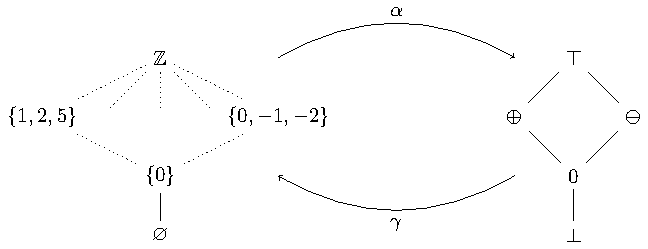
\includegraphics{capitoli/interpretazione-astratta/immagini/reticolo-segni.pdf}
    \caption{Connessione di Galois tra $\wp(\Z)$ e $\set{Sign}$}
    \label{fig:sign}
\end{figure}

\begin{definition}[Connessione di Galois]
Dati due poset $\struct{C, \le}$ e $\struct{A, \preceq}$, la coppia di funzioni $\struct{\alpha, \gamma}$ viene definita \emph{connessione di Galois} e si indica con 
\[ C \galois{\alpha}{\gamma} A \]
dove
\begin{itemize}
    \item[$C$:] insieme detto dominio concreto;
    \item[$\gamma$:] funzione monotona di concretizzazione $\gamma : A \to C$, $\forall c \in C : c \le \gamma(\alpha(c))$;
    \item[$A$:] insieme detto dominio astratto;
    \item[$\alpha$:] funzione monotona di astrazione $\alpha : C \to A$, $\forall a \in A : a \preceq \alpha(\gamma(a))$.
\end{itemize}
\end{definition}

Per mezzo di questo strumento possiamo facilmente trasformare i valori concreti (in input) in valori astratti tramite $\alpha$, effettuare operazioni nel dominio astratto e ri-ottenere i valori nel dominio concreto tramite $\gamma$. 

\begin{example}
Per il dominio di Esempio~\ref{example:sign}, le funzioni $\alpha$ e $\gamma$ sono definite come segue:
\begin{align*}
    \alpha(\varnothing)                                   & = \bot                 &
    \gamma(\bot)                                          & = \varnothing          \\
    \alpha(\{0\})                                         & = 0                    &
    \gamma(0)                                             & = \{ 0 \}              \\
    \alpha(\{ x \mid \min x \ge 0 \}) & = \oplus          &
    \gamma(\oplus)                                        & = \{ x \mid x \ge 0 \} \\
    \alpha(\{ x \mid \max x \le 0 \}) & = \ominus         &
    \gamma(\ominus)                                       & = \{ x \mid x \le 0 \} \\
    \alpha(\{ x \mid \min x < 0 \land \max x > 0\})       & = \top                 &
    \gamma(\top)                                          & = \mathbb{Z}
\end{align*}
\end{example}

\subsection{Inserzione di Galois}\label{sec:galois-i}

Ogni connessione di Galois può diventare un'inserzione di Galois identificando in una classe di equivalenza gli elementi del dominio astratto con la stessa concretizzazione (todo approfondire). Questo processo è chiamato \emph{reduction}. 

\begin{definition}[Inserzione di Galois]
Una connessione di Galois si dice \emph{inserzione di Galois} e si scrive $C \galoiS{\alpha}{\gamma} A$ se $\alpha \circ \gamma = \fun{id}$. Sono equivalenti le seguenti espressioni:
\begin{itemize}
    \item $C \galoiS{\alpha}{\gamma} A$;
    \item $\alpha$ è suriettiva;
    \item $\gamma$ è iniettiva.
\end{itemize}
\end{definition}

Una inserzione di Galois assicura che una volta applicata $\alpha$ su un certo valore perdendo informazioni su esso, se decidiamo di concretizzare e astrarre ancora il tale valore non viene persa alcuna ulteriore informazione.

\section{Operazioni astratte}

Le operazioni che prima effettuavamo nel dominio concreto $C$ ora devono essere effettuate nel dominio astratto A. Data una funzione $f : C \to C$ definiamo $f^{\#} : A \to A$ la sua approssimazione nel dominio astratto. Il modo più immediato di definire $f^{\#}$ è tramite la \emph{best correct approximation}.

\begin{definition}[Best correct approximation]
Data una funzione $f : C \to C$ e una connessione di Galois $C \galois{\gamma}{\alpha} A$, si definisce $f^{\#} = \alpha \circ f \circ \gamma$ la \emph{best correct approximation} di $f$ in $A$.
\end{definition}

Tuttavia vorremmo poter avere il risultato di $f^{\#}$ senza dover eseguire $f$. Possiamo definire in un altro modo $f^{\#}$ e poi dimostrarne la correttezza.

\begin{definition}[Correttezza di una funzione astratta]
Data la connessione di Galois $C \galois{\gamma}{\alpha} A$ tra i due poset $\struct{C, \le}$ e $\struct{A, \preceq}$ ed una funzione $n$-aria $f(c_1, ..., c_n)$, l'operazione $n$-aria $f^{\#}(a_1, ..., a_n)$ è corretta se vale
\[ f(\gamma(a_1), ..., \gamma(a_n)) \le \gamma(f^{\#}(a_1, ..., a_n)) \]
\end{definition}

\begin{example}
Consideriamo la funzione concreta $\fun{add} : \wp(\Z) \times \wp(\Z) \to \wp(Z)$:
\[ \fun{add}(X, Y) = \{ x + y \mid \forall x \in X, \, y \in Y \} \]
Per definire la sua funzione astratta nel dominio dei segni abbiamo più possibilità:
\[ \fun{add}^{\#}_1(s, t) = \alpha(f(\gamma(s), \gamma(t)) \]
oppure
\[ \fun{add}^{\#}_2(s,t) = \begin{array}{r|ccccc}
    s \downarrow; t \rightarrow & \top & \oplus & \ominus & 0       & \bot  \\\hline
    \top                      & \top   & \top   & \top    & \top    & \bot  \\
    \oplus                    & \top   & \oplus & \top    & \oplus  & \bot  \\
    \ominus                   & \top   & \top   & \ominus & \ominus & \bot  \\
    0                         & \top   & \oplus & \ominus & 0       & \bot  \\
    \bot                      & \bot   & \bot   & \bot    & \bot    & \bot  \\
\end{array} \]
oppure 
\[ \fun{add}^{\#}_3(s,t) = \top \]
Tutte e tre le varianti sono corrette. 
\end{example}

\section{Algoritmi fixpoint}


